\documentclass[11pt]{article}
\usepackage[margin=1in]{geometry}
\usepackage{tikz}
\usepackage{algorithm}
\usepackage{algpseudocode}
\usepackage{amsmath}
\usetikzlibrary{arrows.meta,positioning,shapes.multipart}

\title{Barnes--Hut N-Body (2D): Code Map and Pseudocode}
\author{}
\date{}

\begin{document}
\maketitle

\section*{Code Block Graph}

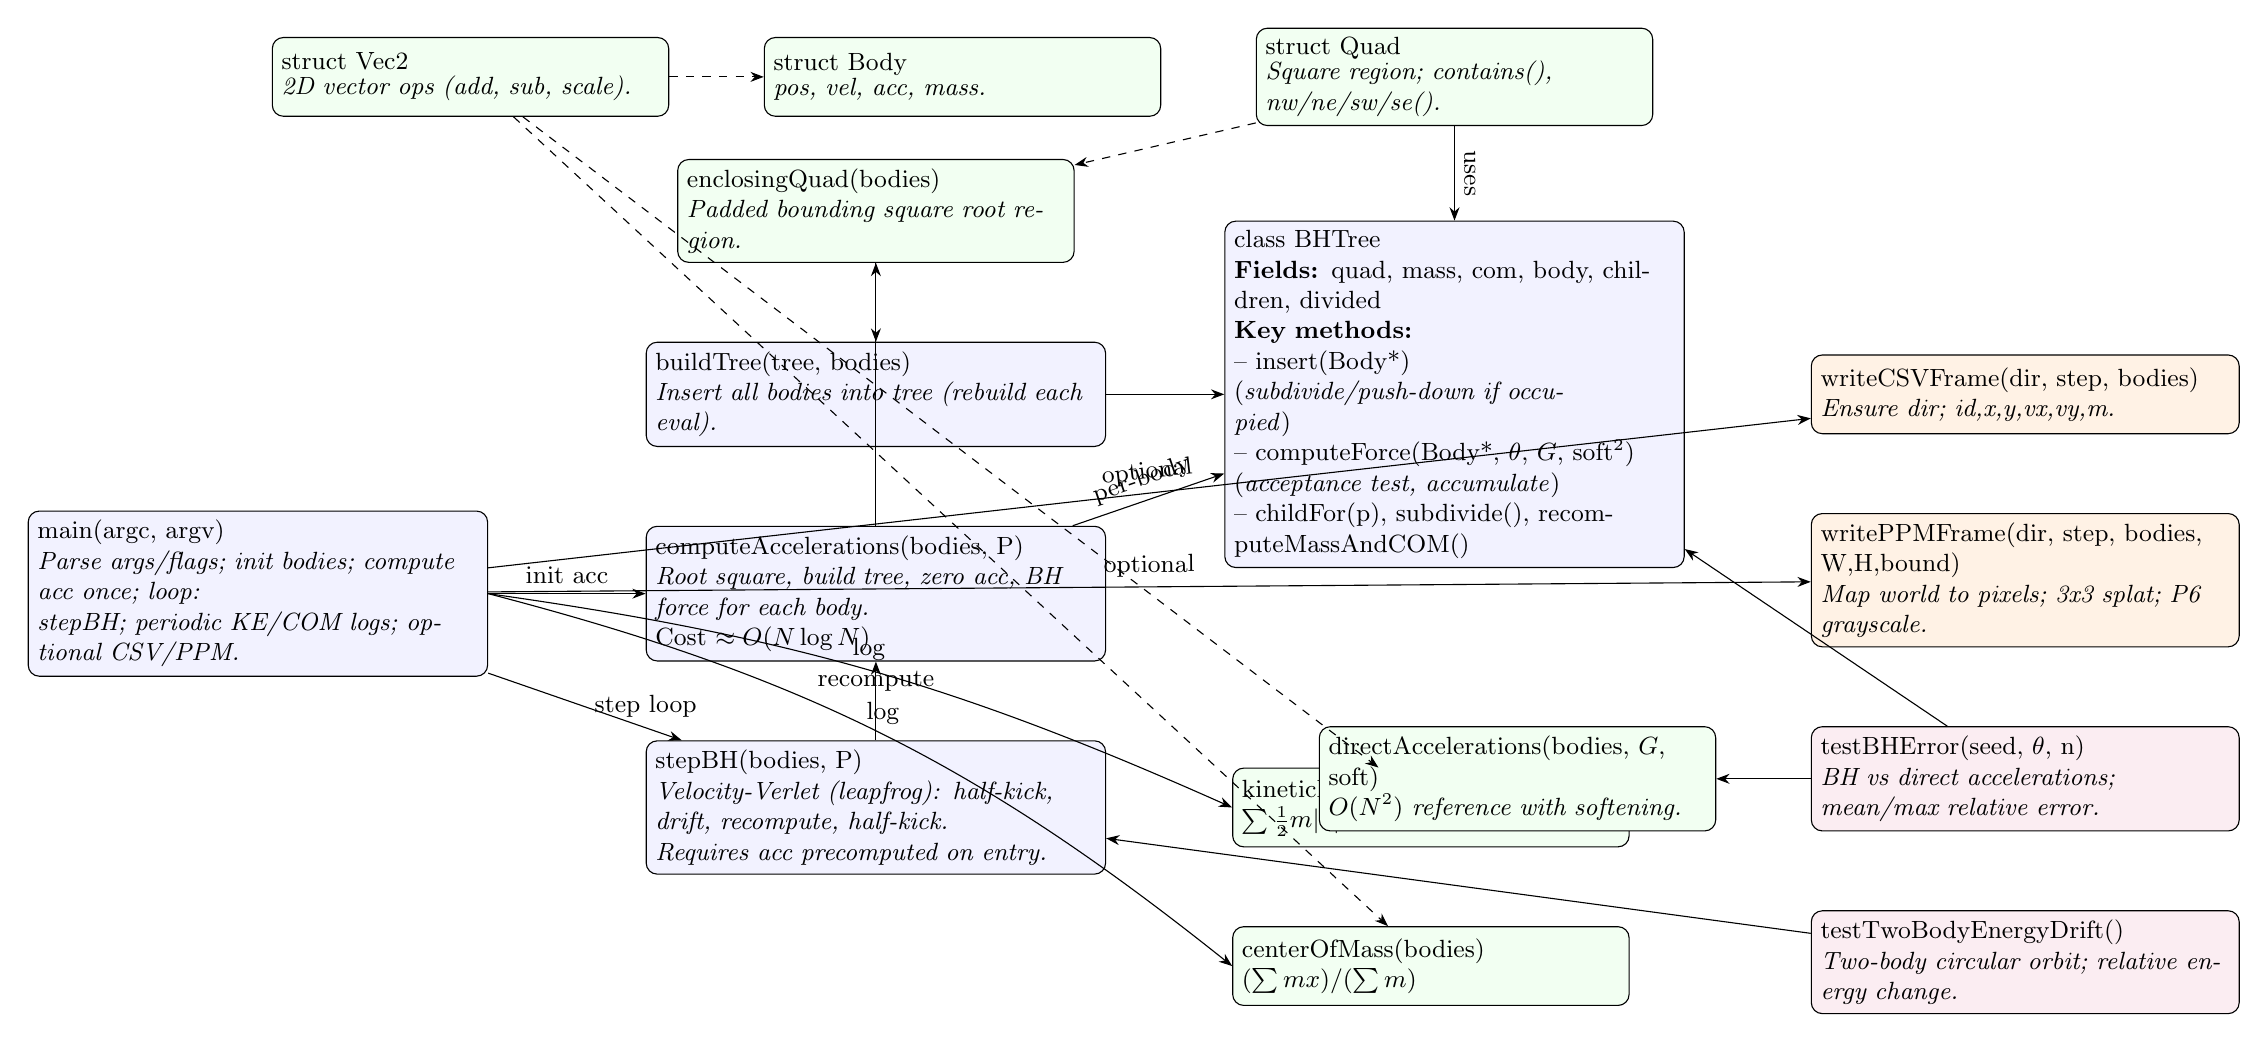
\begin{tikzpicture}[
  node distance=10mm and 12mm,
  >={Stealth},
  font=\small,
  block/.style={rectangle, rounded corners, draw=black, fill=blue!5, align=left, text width=5.6cm, minimum height=1.2cm},
  smallblock/.style={rectangle, rounded corners, draw=black, fill=green!5, align=left, text width=4.8cm, minimum height=1cm},
  io/.style={rectangle, rounded corners, draw=black, fill=orange!10, align=left, text width=5.2cm, minimum height=1cm},
  test/.style={rectangle, rounded corners, draw=black, fill=purple!7, align=left, text width=5.2cm, minimum height=1cm}
]

% Top: basic types
\node[smallblock] (vec2) {struct Vec2\\[-2pt]\textit{2D vector ops (add, sub, scale).}};
\node[smallblock, right=of vec2] (body) {struct Body\\[-2pt]\textit{pos, vel, acc, mass.}};
\node[smallblock, right=of body] (quad) {struct Quad\\[-2pt]\textit{Square region; contains(), nw/ne/sw/se().}};

% Tree
\node[block, below=of quad, yshift=-2mm] (bhtree) {class BHTree\\
\textbf{Fields:} quad, mass, com, body, children, divided\\
\textbf{Key methods:}\\
-- insert(Body*)\ \ \ \ \ \ \ \ \ \ \ \ \ \ \ \ \ \ \ \ \ \ \ (\emph{subdivide/push-down if occupied})\\
-- computeForce(Body*, $\theta$, $G$, soft$^2$)\ (\emph{acceptance test, accumulate})\\
-- childFor(p), subdivide(), recomputeMassAndCOM()};

% Build / accel
\node[block, left=15mm of bhtree] (buildtree) {buildTree(tree, bodies)\\
\textit{Insert all bodies into tree (rebuild each eval).}};
\node[block, below=of buildtree] (accel) {computeAccelerations(bodies, P)\\
\textit{Root square, build tree, zero acc, BH force for each body.}\\
Cost $\approx O(N\log N)$};

% Integrator and helpers
\node[block, below=of accel] (step) {stepBH(bodies, P)\\
\textit{Velocity-Verlet (leapfrog): half-kick, drift, recompute, half-kick.}\\
\textit{Requires acc precomputed on entry.}};
\node[smallblock, right=16mm of step] (diag1) {kineticEnergy(bodies)\\\textit{$\sum \tfrac12 m|v|^2$}};
\node[smallblock, below=of diag1] (diag2) {centerOfMass(bodies)\\\textit{$(\sum m x)/(\sum m)$}};

% IO
\node[io, right=16mm of bhtree] (csv) {writeCSVFrame(dir, step, bodies)\\
\textit{Ensure dir; id,x,y,vx,vy,m.}};
\node[io, below=of csv] (ppm) {writePPMFrame(dir, step, bodies, W,H,bound)\\
\textit{Map world to pixels; 3x3 splat; P6 grayscale.}};

% Tests
\node[test, below=of ppm] (testerr) {testBHError(seed, $\theta$, n)\\
\textit{BH vs direct accelerations; mean/max relative error.}};
\node[test, below=of testerr] (testeng) {testTwoBodyEnergyDrift()\\
\textit{Two-body circular orbit; relative energy change.}};

% Direct ref
\node[smallblock, left=of testerr] (direct) {directAccelerations(bodies, $G$, soft)\\
\textit{$O(N^2)$ reference with softening.}};

% enclosing quad
\node[smallblock, above=of buildtree] (enclose) {enclosingQuad(bodies)\\
\textit{Padded bounding square root region.}};

% main
\node[block, left=of accel, xshift=-8mm] (main) {main(argc, argv)\\
\textit{Parse args/flags; init bodies; compute acc once; loop:}\\
\textit{stepBH; periodic KE/COM logs; optional CSV/PPM.}};

% Edges (calls / uses)
\draw[->] (quad) -- node[midway, above, sloped] {\small uses} (bhtree);
\draw[->] (enclose) -- (buildtree);
\draw[->] (buildtree) -- (bhtree);
\draw[->] (accel) -- node[midway, above, sloped] {\small per-body} (bhtree);
\draw[->] (main) -- node[midway, above] {\small init acc} (accel);
\draw[->] (main) -- node[midway, right] {\small step loop} (step);
\draw[->] (step) -- node[midway, above] {\small recompute} (accel);
\draw[->] (main.east) to[bend left=8] node[midway, above] {\small log} (diag1.west);
\draw[->] (main.east) to[bend left=12] node[midway, above] {\small log} (diag2.west);
\draw[->] (main) -- node[midway, above, sloped] {\small optional} (csv);
\draw[->] (main) -- node[midway, above, sloped] {\small optional} (ppm);
\draw[->] (testerr) -- (direct);
\draw[->] (testerr) -- (bhtree);
\draw[->] (testeng) -- (step);
\draw[->] (accel) -- (enclose);

% Basic types influences (light connectors)
\draw[->, dashed] (vec2) -- (body);
\draw[->, dashed] (vec2) -- (diag1);
\draw[->, dashed] (vec2) -- (diag2);
\draw[->, dashed] (quad) -- (enclose);

\end{tikzpicture}

\bigskip

\section*{Core Pseudocode}

\begin{algorithm}[H]
\caption{computeAccelerations(bodies, P)}
\begin{algorithmic}[1]
\State rootQuad $\gets$ enclosingQuad(bodies)
\State tree $\gets$ BHTree(rootQuad)
\State buildTree(tree, bodies)
\State soft2 $\gets P.\text{softening}^2$
\ForAll{b in bodies}
  \State b.acc $\gets (0,0)$
  \State tree.computeForce(\&b, $P.\theta$, $P.G$, soft2)
\EndFor
\end{algorithmic}
\end{algorithm}

\begin{algorithm}[H]
\caption{stepBH(bodies, P) \ \ (Velocity--Verlet / Leapfrog)}
\begin{algorithmic}[1]
\State $h \gets 0.5 \cdot P.dt$
\ForAll{b in bodies} \Comment{half-kick}
  \State b.vel $\gets$ b.vel $+$ $h \cdot$ b.acc
\EndFor
\ForAll{b in bodies} \Comment{drift}
  \State b.pos $\gets$ b.pos $+$ $P.dt \cdot$ b.vel
\EndFor
\State computeAccelerations(bodies, P) \Comment{forces at new positions}
\ForAll{b in bodies} \Comment{half-kick}
  \State b.vel $\gets$ b.vel $+$ $h \cdot$ b.acc
\EndFor
\end{algorithmic}
\end{algorithm}

\begin{algorithm}[H]
\caption{BHTree.insert(b)}
\begin{algorithmic}[1]
\If{not quad.contains(b.pos)} \State \Return \EndIf
\If{not divided and body = null and mass = 0}
  \State body $\gets$ b; mass $\gets$ b.mass; com $\gets$ b.pos; \Return
\EndIf
\If{not divided} \Comment{occupied leaf $\Rightarrow$ subdivide and push down}
  \State subdivide()
  \If{body $\neq$ null}
    \State childFor(body.pos).insert(body)
    \State body $\gets$ null
  \EndIf
\EndIf
\State childFor(b.pos).insert(b)
\State recomputeMassAndCOM()
\end{algorithmic}
\end{algorithm}

\begin{algorithm}[H]
\caption{BHTree.computeForce(b, $\theta$, $G$, soft2)}
\begin{algorithmic}[1]
\If{mass $= 0$} \State \Return \EndIf
\If{not divided} 
  \If{body = null or body == b} \State \Return \EndIf
  \State addAccelFromCOM(b, com, mass, $G$, soft2); \Return
\EndIf
\State size $\gets 2 \cdot$ quad.half
\State $d \gets \|\text{com} - b.pos\| + \varepsilon$ \Comment{tiny $\varepsilon$ avoids 0}
\If{size / d $< \theta$}
  \State addAccelFromCOM(b, com, mass, $G$, soft2)
\Else
  \ForAll{child in \{nw, ne, sw, se\}}
    \If{child exists} \State child.computeForce(b, $\theta$, $G$, soft2) \EndIf
  \EndFor
\EndIf
\end{algorithmic}
\end{algorithm}

\begin{algorithm}[H]
\caption{Potential helper formulas}
\begin{algorithmic}[1]
\State Softened pair acceleration from point mass $m$ at $p$ on body at $x$
